\documentclass[10pt,twocolumn,letterpaper]{article}

\usepackage{cvpr}
\usepackage{times}
\usepackage{epsfig}
\usepackage{graphicx}
\usepackage{amsmath}
\usepackage{amssymb}

% Include other packages here, before hyperref.

% If you comment hyperref and then uncomment it, you should delete
% egpaper.aux before re-running latex.  (Or just hit 'q' on the first latex
% run, let it finish, and you should be clear).
\usepackage[breaklinks=true,bookmarks=false]{hyperref}

\cvprfinalcopy % *** Uncomment this line for the final submission

\def\cvprPaperID{****} % *** Enter the CVPR Paper ID here
\def\httilde{\mbox{\tt\raisebox{-.5ex}{\symbol{126}}}}

% Pages are numbered in submission mode, and unnumbered in camera-ready
%\ifcvprfinal\pagestyle{empty}\fi
\setcounter{page}{4321}
\begin{document}

%%%%%%%%% TITLE
\title{Spatio-Temporal reconstruction of Rigid objects from multiple cameras}


\maketitle
%\thispagestyle{empty}

%%%%%%%%% ABSTRACT
\begin{abstract}
Multi camera based understanding of dynamic scenes from unsynchronized images is a challening problem in reconstruction. We propose a solution to the problem of 3D reconstruction of multiple moving rigid objects from unsynchronized multiple cameras. Most of the reconstruction piplines leverage reconstruction using reprojection error of features, we propose a novel semantic features pipeline and object based feature tracking for reconstruction of dynamic objects. We leverage multiple rigid object constraints in a bundle adjustment framework to improve the reconstuction. \end{abstract}
\section{INTRODUCTION}
We propose dynamic reconstruction of rigid objects from multiple unsynchronized and in the wild captured cameras. The main contributions of the algorithm are:
\begin{enumerate}
\item Novel instance keypoint detection pipeline for reconstruction of moving objects.
\item Constraint Bundle adjustment for reconstruction of dynamic rigid moving objects from viwed from multiple cameras. 
\item End-to-End dense recosntruction of rigid objects from multiple unsynchronized cameras.
\end{enumerate}
\section{METHOD}
We Follow the basic pipeline of reconstcruion i.e. feature detection and tracking, correspodence of the keypoint across views and then bundle adjustment for accurate reconstruction of the 3d points. In each of the segments of the pipeline we incorporate geometric and semantic information of the objects for better reconstruction. We propose instance keypoint segmentation for better feature detection of important points on the rigid object. 
We first formulate the problem statement for the problem. Lets assume $N$ video cameras observing $P$ 3d points over time $X^p(t)$ and their 2D projection $x^p_n(f)$ on camera $p$ and frame $f$ is given as:

\begin{align*}
 \begin{bmatrix} x_n^p(f) \\ 1  \end{bmatrix} = K_n(f)[R_n(f) | T_n(f)] \begin{bmatrix} X_n(f) \\ 1  \end{bmatrix}
\end{align*} 

where $K_n(f)$ is the intrisic camera matrix, $R_n(f)$ and $T_n(f)$ are the relative camera rotation and translation, respectively. We denote this transformations $x_c^n(f) = P_n(f,X^n(t))$
%-------------------------------------------------------------------------
\subsection{Instance Aware Keypoint detection}
Given a images with multiple moving objects. The amount of objects which can move can be sorted into a small set of categories like cars and humans. We propose a instance keypoint detection on these categories for improving the reconstruction of these objects. We leverage deep learning framwork for fast and accurate detection of semantic features in images. We pass the input image through a detection pipeline and each detected bounding box is passed through a object specific keypoint detection pipeline for computation of semantic features in an image.  

\subsection{Object aware keypoint tracking}
Tracking of keypoints has generally been considered as a search problem over the image space for features of similar shape in adjustcent images. Semantic aware tracking correspondences to tracking of the important parts using the knowledge of the object i.e. the keypoints on the wheels are tracked by finding the correspondences of cars overtime. This gives a better tracks of the keypoints and longer correpondeces compared to the feature based tracking methods. 

\subsection{Correspondence across views}
We currently have tracks of objects and thier respective keypoints in each individual video for all videos of the scene. For accurate reconstruction of objects from multiple views we need to find corrospondences across views. We propose a object specific bundle adjustment for finding correspondes across views. Lets assume we have $h$ object proposals in $N$ videos at time $t$. The problem of correspondence is finding $g$, where $g \subset h$ object bounding boxes which belong to the same object. Since there is a spatial constraint on the bounding boxes over multiple views, Fig \ref{fig:corr} shows the bundle adjustment we use to find correspondes across views. We propose a ransac based methodology for finding correspondenses across views and minimize the following reprojection error:

\begin{equation}
  	E_r =\sum_{n=1}^{N} \sum_{p=1}^P \sum_{f=1}^{F_n} V_n^p(f) ||P_n(f,X^p(t)) - x_n^p(f)||^2
\end{equation}
   
where $E_r$ is the image reprojection error, $V_n^p(f)$ is a binary indicator of the visibilty of the keypoint. We add additional constraints like symmetry and the length of different joints of the object for accurate fitting of the rigid object in 3D. A joint in 3d can be defined as the difference of the 3D points between the centers of the joint. We define a joint as $J(p1,p2) = X^{p1}(t) - X^{p2}(t) $ where p1 and p2 correspond to different parts of the rigid object which are linked. 

\begin{equation}
  	E_l = \sum_{r=1}^R ||J(r) - E(J(r))||^2  
\end{equation}

where $E(J(r))$ is the mean length of joint $r$. We model the symmetry constraint in the budle adjustment for better reconstruction of rigid objects.
\begin{equation}
  	E_j = \sum_{q = 1}^Q ||J(q) - J(S(q))||^2
\end{equation}

where $S(q)$gives the corresponding symmetric joint of $q$ i.e. if q is the joint connecting the left wheels of a car S(q)is the joint connecting the right wheels of the car.

\subsection{Spatio-Temporal Bundle Adjustment}
Once we have the correspondences across cameras and views, We get the fit a motion model based rigid object over time. The formulation is given by:

\begin{equation}
 E_{st} = \sum_{t=1}^T w_r E_r + w_j E_j + w_l E_l + w_m E_m 
\end{equation}

where $w$ represents the weights of each term in the bundle adjustment. $E_m$ is defined as the motion prior over the trajectory of the points.

\begin{equation}
E_m = \sum_{p =1 }^P \sum_{i = 1}^{T^n -1} ||\frac{X^p(t^{i+1}) - X^p(t^{i})}{t^{i+1} - t^{i}}||^2 (t^{i+1} - t^{i})
\end{equation}
\begin{figure}
  \centering
    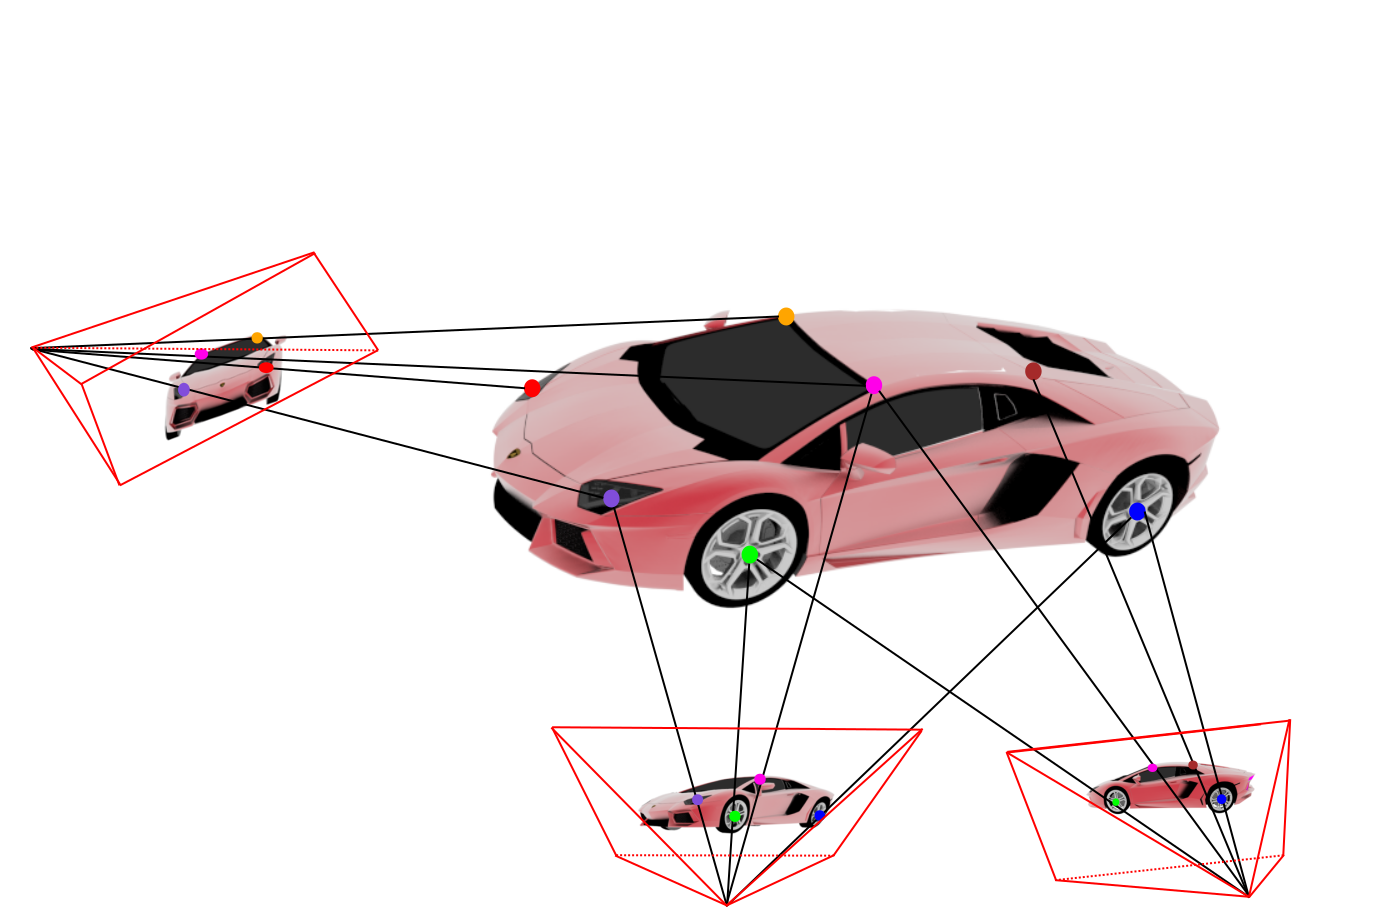
\includegraphics[width=0.4\textwidth]{images/corr}
  \caption{The picture depicts the projection of 3D keypoints of car onto thier respective videos}
  \label{fig:corr}
\end{figure}


\end{document}
